\documentclass[preprint,12pt]{elsarticle}
\usepackage{lmodern}
\usepackage[T1]{fontenc}
\usepackage{microtype}
\usepackage{graphicx}
\usepackage{booktabs}
\usepackage{array}
\usepackage{amsmath,amssymb}
\usepackage{xcolor}
\usepackage{hyperref}
\usepackage{subcaption}
\usepackage{enumitem}
\usepackage{siunitx}
\usepackage{caption}
\usepackage{url}
\usepackage{multirow}
\usepackage{float}
\hypersetup{colorlinks=true,linkcolor=black,citecolor=black,urlcolor=blue}
\biboptions{numbers,sort&compress}

\begin{document}
\begin{frontmatter}
\title{When Missing Days Change Photovoltaic Decisions: Four-Source Reliability Surfaces and Critical Gain Sensitivity}
\author{Anonymous for pre-submission author review}
\begin{abstract}
Missing observations in photovoltaic (PV) monitoring are commonly summarized by a missing-data rate or reconstruction error. We instead audit whether a multi-candidate PV shortlist changes when contiguous whole days are deleted without imputation. Within each admitted calendar month, candidates within margin $q$ of the leader's normalized yield are retained; we stress $q\in\{0,2.5,5,7.5,10\%\}$ and gaps of up to seven days, retaining at least ten days. The original frozen design covers 25 PROPRE.MA, seven EURAC, and 79 MORE-EU source-months. A retrospective fourth-source check uses three complete months of three co-roof inverters from the public HKUST rooftop archive, with source-derived module capacities and paired site/inverter measurements. At $q=5\%$ and gaps no longer than three days, the corresponding fragile-month counts are 3/25, 1/7, 45/79, and 0/3; these nonexchangeable fractions are reported separately. The HKUST shortlist remained unchanged through seven-day omissions at $q=5\%$, whereas one of its three months changed at $q=10\%$ and $L\leq7$. Over 93 complete HKUST Library days, the site-power integral and sum of inverter-power integrals differed by a median absolute relative 0.428\% (95th percentile 0.994\%), supporting aggregate source consistency, not individual inverter calibration. A baseline-preserving hypothetical gain stress identifies critical per-inverter gain envelopes of 0.469\%, 2.025\%, and 1.827\% across the three HKUST Library months. No distribution or covariance of instrument errors is calibrated. The study shows why missing-data percentage alone cannot certify a discrete PV decision and why decision margin, omission structure, and source measurement boundaries must be reported together.
\end{abstract}
\begin{keyword}
photovoltaic monitoring \sep missing data \sep decision reliability \sep contiguous gaps \sep set-valued decisions \sep critical gain margin \sep no imputation
\end{keyword}
\end{frontmatter}

\section{Introduction}
Field PV monitoring is intrinsically incomplete. Communication outages, logger failures, inverter downtime, sensor faults, time-base irregularities, and maintenance can remove or invalidate observations before a performance indicator is computed. Established PV data-quality work therefore emphasizes detection, filtering, reconstruction, and careful treatment of missing values. Koubli et al. reconstructed missing PV monitoring data to recover performance-ratio information \cite{koubli2016}; Livera et al. developed a structured data-quality and reconstruction pipeline and showed that performance and reliability analytics can be sensitive to missingness rate and treatment \cite{livera2021}; IEA PVPS guidance similarly treats missing-data handling as a prerequisite for credible technical key performance indicators \cite{ieapvps2024}. More recent work has continued to develop mask-aware repair policies for incomplete PV records \cite{wang2026}, while long-term performance-loss studies have explicitly tested the effect of sporadic gaps on continuous estimands such as performance loss rate \cite{quest2025}.

Those studies ask how well a missing continuous signal or downstream continuous metric can be recovered or estimated. Many engineering comparisons, however, end with a \emph{discrete} decision: retain several candidates within a tolerance of the leader, exclude a candidate, or select a set for further engineering review. A small error in a continuous performance metric need not change that set, whereas a modest removal of high-leverage days can change the set when candidates lie near its boundary. Conversely, substantial missingness can leave the set unchanged when candidates are well separated. A missing-data percentage alone therefore need not identify the reliability of the discrete decision built on the data.

The general idea of testing a conclusion by removing observations is not new. Minimal case-removal and fragility ideas appear in model comparison and decision audits \cite{alzhrani2026}, automatic finite-sample robustness assessment \cite{giordano2026}, training-set removal analyses \cite{yang2023}, and ranking-stability research \cite{liang2025}. The contribution of the present work is deliberately narrower: we adapt this logic to a PV monitoring decision object and ask what the retained observations support \emph{without imputing deleted whole-day energy}. We further distinguish the decision margin from the temporal structure of missingness by mapping a two-dimensional reliability surface over shortlist margin $q$ and contiguous gap length $L$.

Three originally frozen field sources differ in provenance and interpretation. PROPRE.MA provides multi-site technology comparisons in Morocco \cite{bennouna2019}; EURAC provides public multi-system measurements \cite{eurac2026}; and MORE-EU provides normalized output for 14 arrays of one solar park \cite{moreeu2026}. We now add a \emph{retrospective}, separately gated fourth-source demonstration using co-located inverter and site-power channels from the HKUST campus archive in Hong Kong \cite{lin2025,hkust2024}. The original three-source analysis remains locked; HKUST was not part of its frozen cohort. None of the source-month fractions is pooled or interpreted as independent field-failure trials. This extension tests whether the decision-audit interpretation and its evidence boundary survive another measurement chain, not whether performance of technologies or installations can be compared across sites.

The resulting paper has four objectives:
\begin{enumerate}[leftmargin=1.5em]
    \item define a transparent PV candidate-set audit that does not reconstruct missing whole-day energy;
    \item separate the shortlist decision margin $q$ from contiguous missing-gap length $L$;
    \item evaluate the frozen surface on three original field sources and a retrospective, source-qualified fourth observed-inverter subset without pooling their frequencies; and
    \item identify claim boundaries that prevent a data-quality sensitivity result from being misread as technology superiority, procurement failure, or calibrated probability.
\end{enumerate}

\section{Methods}
\subsection{Decision object}
For calendar month $m$, let $D_m$ be the set of admitted observed days and let $Y_{m,j}(D)$ denote accumulated normalized yield for candidate $j$ over a retained day set $D\subseteq D_m$. The normalization is source-specific: system-specific STC denominators are used where defensible, whereas the MORE-EU source already reports normalized array output. For a declared relative decision margin $q\in[0,1)$, the candidate shortlist is
\begin{equation}
S_m(q;D)=\left\{j:\;Y_{m,j}(D)\geq (1-q)\max_k Y_{m,k}(D)\right\}.
\label{eq:shortlist}
\end{equation}
The full-data reference set is $S_m(q;D_m)$. The value $q$ is a decision resolution. It is not a sensor-accuracy tolerance, confidence level, or probability.

\subsection{Contiguous whole-day deletion stress}
A contiguous gap beginning at calendar position $s$ and lasting $\ell$ whole days is denoted $G_m(s,\ell)$. Deleted days are not reconstructed, predicted, or redistributed. For a maximum tested gap length $L$, define the month-level indicator
\begin{equation}
F_m(q,L)=\mathbf{1}\left[\exists\;\ell\leq L,\;s:\;S_m(q;D_m\setminus G_m(s,\ell))\neq S_m(q;D_m)\right],
\label{eq:fragile}
\end{equation}
subject to at least ten retained days. The source-level descriptive surface is
\begin{equation}
R_{\mathcal{D}}(q,L)=\frac{1}{M_{\mathcal{D}}}\sum_{m=1}^{M_{\mathcal{D}}}F_m(q,L),
\label{eq:surface}
\end{equation}
where $M_{\mathcal{D}}$ is the number of admitted complete months in source $\mathcal{D}$. Equation~\eqref{eq:surface} is a descriptive fraction within a source, not a population probability. Months share systems, seasons, and operational histories and are not treated as independent replications.

The original three-source design was frozen before inspecting the combined surface: $q\in\{0,0.025,0.05,0.075,0.10\}$; $L=1,\ldots,7$ days; at least ten retained days. The $q=5\%$ row was retained as a continuity point with prior project stages, not because it maximized an effect.

\subsection{Source admission and estimands}
Table~\ref{tab:data} summarizes the three original frozen cohorts and one retrospective HKUST subset. Detailed source-admission rules, including HKUST's native source clock and paired site/inverter channel check, are in the Supplementary Material.

\begin{table}[H]
\centering
\caption{Source-specific cohorts and decision objects. Counts are source-months, not independent climate trials.}
\label{tab:data}
\small
\begin{tabular}{p{2.2cm}p{1.5cm}p{4.2cm}p{6.0cm}}
\toprule
Source & Months & Decision object & Main admission/interpretation boundary \\
\midrule
PROPRE.MA & 25 & Three-technology normalized-yield shortlist & Complete, boundary-stable primary months from the source-locked counter reconstruction. Raw donor files remain restricted; no missing daily energy is filled. \\
EURAC & 7 & Four observed-system DC specific-yield shortlist & Public 2015 data; four systems with defensible module count and STC capacity; common-timestamp DC $P_{mpp}$ integration and a 95\% daily irradiance-support gate. Mounting geometry is not fully specified, so the estimand is observed-system comparison, not intrinsic technology efficiency. \\
MORE-EU & 79 & Normalized 14-array output shortlist & Public 15-minute normalized array output; a day is admitted only with exactly 96 rows and 96 unique quarter-hour labels. Source-clock 23/25-hour days are excluded rather than rescaled. \\
HKUST (new) & 3 & Three observed co-roof inverter AC-yield/STC shortlist & One Library roof; complete 144-sample source-daylight records at five-minute cadence with source-traced DC-STC denominators; retrospective external check, not device calibration. \\
\bottomrule
\end{tabular}
\end{table}

\paragraph{PROPRE.MA.} The original Moroccan program installed comparable three-technology PV systems across 20 sites and has already been analyzed for multi-site relative yield and data-quality correction \cite{bennouna2019}. The present cohort is not a re-ranking of the 20-site program. It uses 25 complete months retained after source identity, cumulative-counter, and boundary checks developed before this manuscript. System/configuration-specific STC denominators are preserved. Because raw donor data are restricted, the paper reports derived month-level decision evidence rather than redistributing original observations.

\paragraph{EURAC.} The public EURAC archive is identified by DOI and checksum \cite{eurac2026}. Four primary systems had defensible numeric module counts and STC ratings in the supplied metadata: Trina poly-Si (2070~W), SunPower mono-Si (1200~W), Sanyo HJT (3870~W), and Wurth CIGS (1050~W). First Solar was excluded from the primary normalized comparison because total system STC could not be defensibly reconstructed from the supplied metadata. Daily DC energy was integrated from exact common 15-minute timestamps. A day was admitted only when common timestamps retained at least 95\% of the day's positive recorded irradiance support. Seven calendar months met the complete-month gate. Tilt, azimuth, tracking, and other configuration details are not fully resolved in the supplied metadata, so these are observed-system decisions.

\paragraph{MORE-EU.} The public MORE-EU repository describes normalized 15-minute output for 14 arrays of a solar park over 2016--2023 \cite{moreeu2026}. The analysis uses the pinned public Git blob of \texttt{Array Power.csv}. A strict source-calendar gate requires 96 rows and 96 unique quarter-hour labels for every day of an admitted month. Seventy-nine months satisfy this requirement. The 14 arrays are not relabeled as 14 technologies.

\paragraph{HKUST retrospective extension.} The original public HKUST dataset covers 60 rooftop PV installations, but this comparison admits only three inverters at the Library roof \cite{lin2025,hkust2024}. Each admitted day has exactly 144 unique finite five-minute inverter power samples over the source's recorded 06:00--17:55 daylight window; July 2022, May 2023, and July 2023 pass the complete-calendar-month gate for all three devices. Original Brick/RDF metadata gives their module DC STC as $156\times370=57{,}720$~W, $152\times370=56{,}240$~W, and $152\times370=56{,}240$~W, summing to the published $170{,}200$~W Library rating. For observed retained days $D$, the compared specific-yield proxy is $\sum_{t\in D}P_j(t)\Delta t/P_{j,\mathrm{STC}}$, with equal $\Delta t=5$ minutes. These candidates are \emph{observed inverters}, not technologies or intrinsic efficiencies. Other HKUST roof groups with unresolved station/inverter rating bases or electrical-data alerts were not promoted to the primary extension. HKUST was identified and studied \emph{after} the three-source R22 freeze; its analysis is explicitly retrospective, not a blinded prospective external validation.

\subsection{Analysis and reproducibility checks}
No hypothesis test or confidence interval is attached to $R_{\mathcal{D}}(q,L)$ because the months are serially and structurally dependent and because the four source-specific decision objects have different candidate semantics. The analysis instead emphasizes deterministic re-computation, source-specific denominators, and explicit sensitivity dimensions.

A required cross-stage verification was specified before accepting the expanded surface: at $q=5\%$ and $L\leq3$ days, the expanded analysis had to reproduce the locked structured-gap counts from the preceding novelty-gate stage. The required values were 3/25 for PROPRE.MA, 1/7 for EURAC, and 45/79 for MORE-EU. All three were reproduced exactly. The later HKUST extension was evaluated with the \emph{same} frozen $q\times L$ definitions, without changing the original cohort memberships or any original numerical result. A public reproducibility repository releases the locked publication tables and verification scripts and reruns these checks before rebuilding the figures and review PDFs (see Data and code availability).

\section{Results}
\subsection{A single missing-data percentage does not summarize decision reliability}
At $q=5\%$, the three originally frozen sources show markedly different sensitivity to contiguous missing days; the later HKUST check is shown separately in the same comparison table (Table~\ref{tab:q5}). One-day gaps change the declared shortlist in 1/25 PROPRE.MA months, 1/7 EURAC months, and 35/79 MORE-EU months. Extending the allowed contiguous gap to three days increases the corresponding counts to 3/25, 1/7, and 45/79; at seven days they are 4/25, 1/7, and 51/79. These fractions are source-descriptive only.

\begin{table}[H]
\centering
\caption{Primary continuity point $q=5\%$: cumulative months for which at least one contiguous gap of length $\leq L$ changes the shortlist.}
\label{tab:q5}
\begin{tabular}{lrrrr}
\toprule
Dataset & Admitted months & $L\leq1$ day & $L\leq3$ days & $L\leq7$ days \\
\midrule
PROPRE.MA & 25 & 1 (4.0\%) & 3 (12.0\%) & 4 (16.0\%) \\
EURAC & 7 & 1 (14.3\%) & 1 (14.3\%) & 1 (14.3\%) \\
MORE-EU & 79 & 35 (44.3\%) & 45 (57.0\%) & 51 (64.6\%) \\
HKUST Library\textsuperscript{a} & 3 & 0 (0.0\%) & 0 (0.0\%) & 0 (0.0\%) \\
\bottomrule
\end{tabular}
\begin{flushleft}\footnotesize\textsuperscript{a} Retrospective, single-roof observed-inverter source; not one of the original three-source cohorts.\end{flushleft}
\end{table}

This result does not imply that MORE-EU is intrinsically less reliable than the other sources. Candidate counts, normalized responses, operating history, and source structure differ. The result instead demonstrates why a rate-only threshold cannot be transported from one decision object to another without stating what the decision is.

\subsection{Reliability is a joint $q\times L$ surface}
Figures~\ref{fig:proprema}--\ref{fig:moreeu} show the original three predeclared surfaces; the smaller retrospective HKUST surface is tabulated separately in Supplementary Table~S4. Increasing $L$ can only expand the set of admissible deletions and therefore makes $R_{\mathcal D}(q,L)$ nondecreasing in $L$ for fixed $q$. The behavior across $q$ is different: changing $q$ moves the boundary of the shortlist itself, and the fragile fraction is non-monotonic in $q$ in all three datasets at seven-day support.

\begin{figure}[H]
\centering
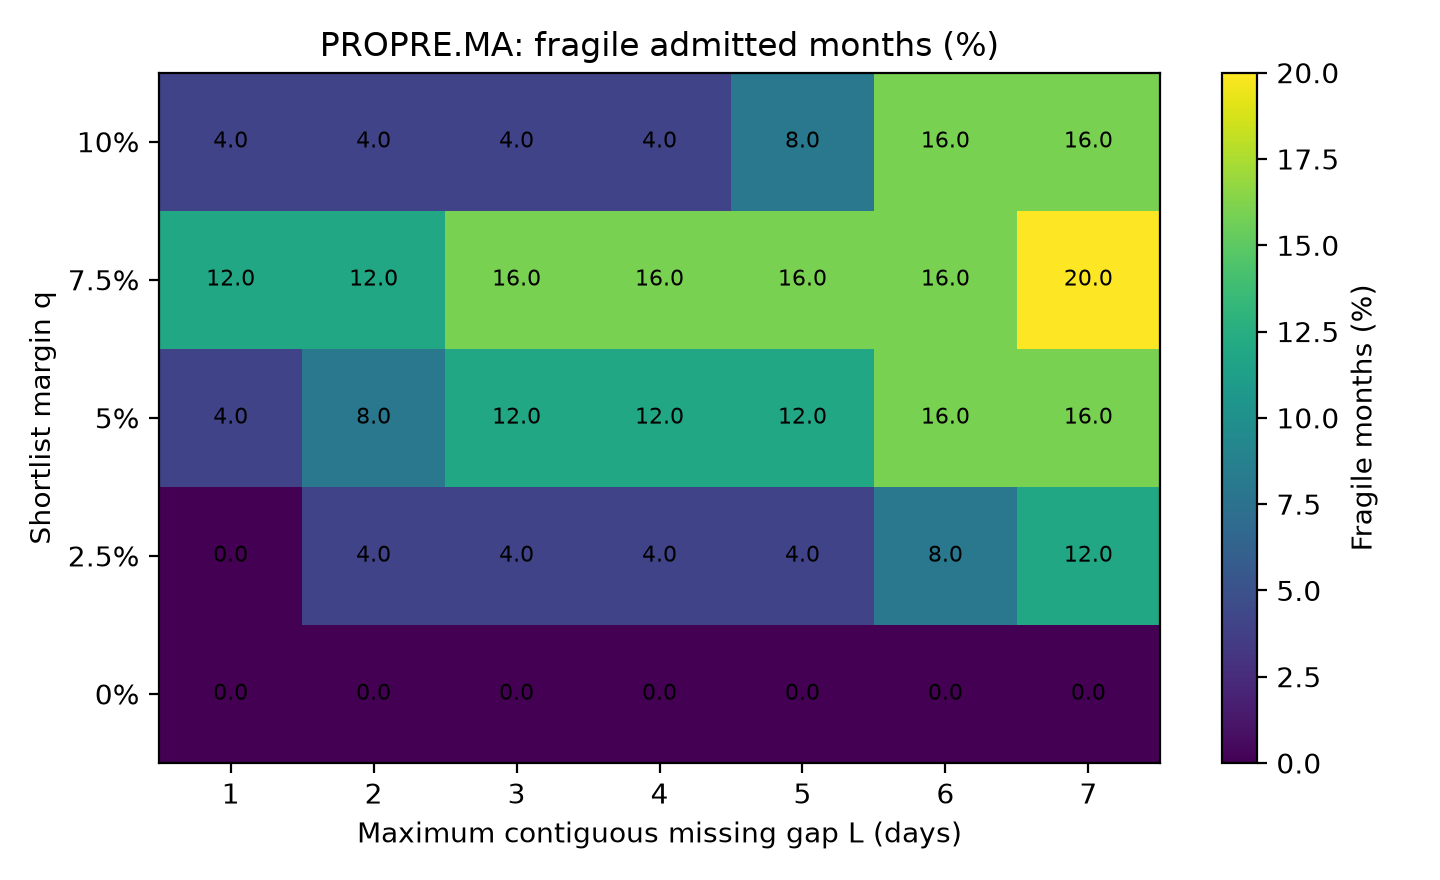
\includegraphics[width=0.82\textwidth]{figures/R22_SURFACE_PROPREMA.png}
\caption{PROPRE.MA decision-reliability surface (25 admitted months). Each cell is the fraction of admitted months for which at least one contiguous whole-day gap of length no greater than $L$ changes the shortlist defined by $q$.}
\label{fig:proprema}
\end{figure}

\begin{figure}[H]
\centering
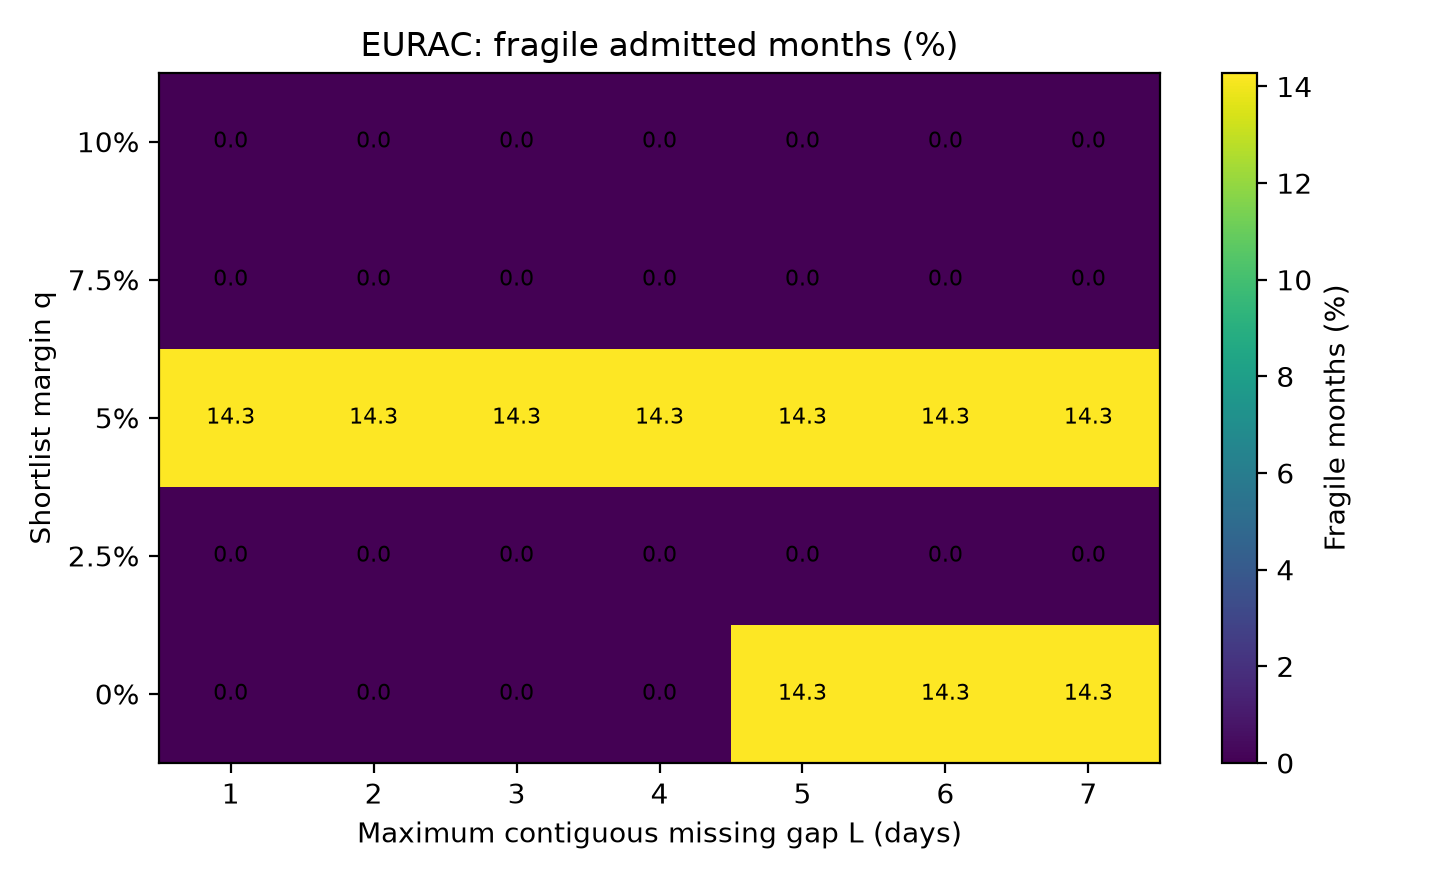
\includegraphics[width=0.82\textwidth]{figures/R22_SURFACE_EURAC.png}
\caption{EURAC observed-system decision-reliability surface (7 admitted months). The small cohort is shown as external directional evidence, not a stable frequency estimate.}
\label{fig:eurac}
\end{figure}

\begin{figure}[H]
\centering
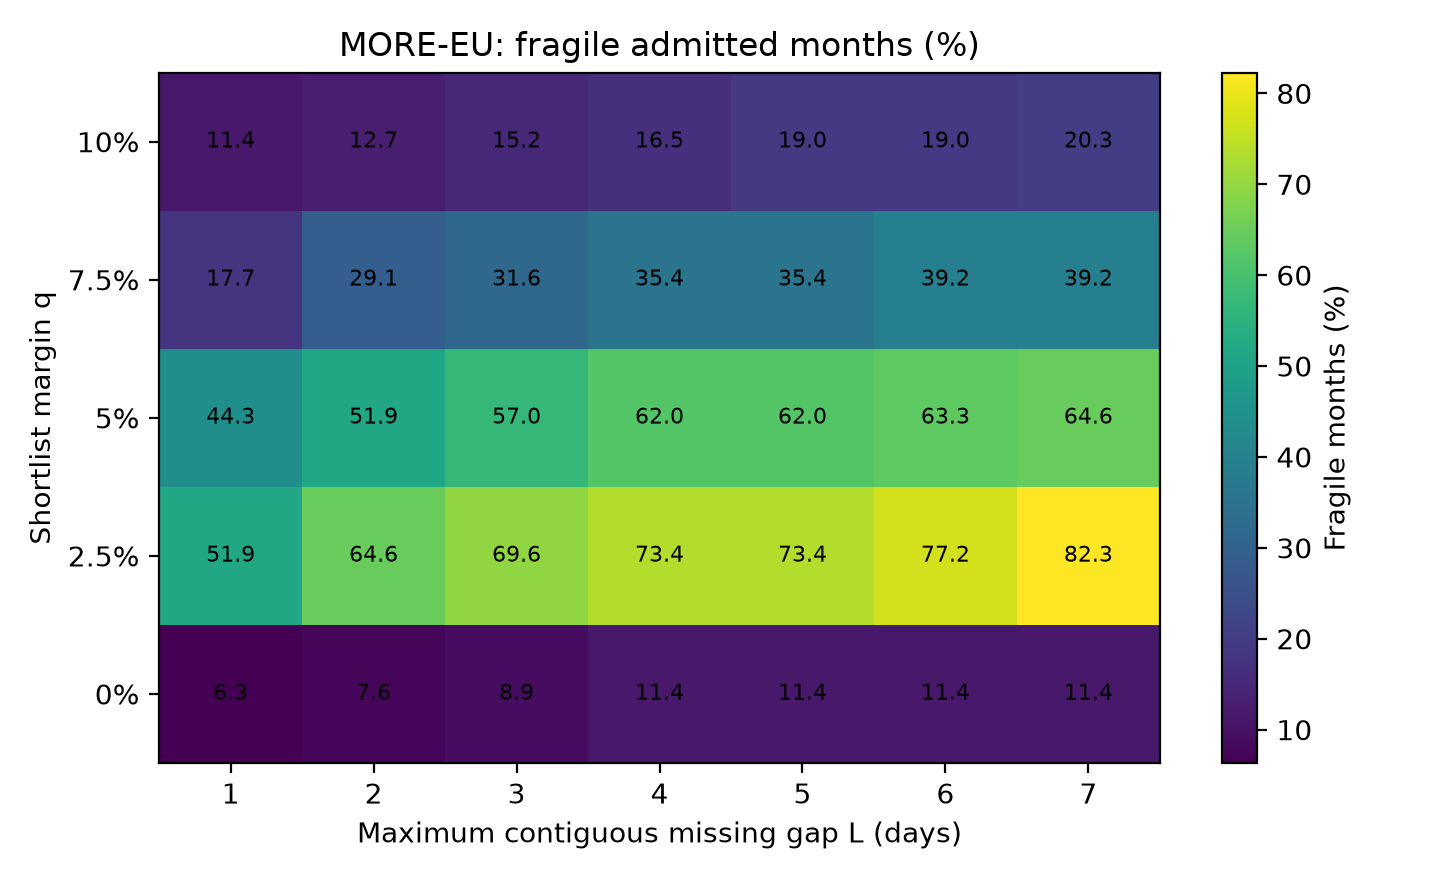
\includegraphics[width=0.82\textwidth]{figures/R22_SURFACE_MORE_EU.png}
\caption{MORE-EU normalized-array decision-reliability surface (79 admitted months). The months are serially dependent observations from one plant; colors are descriptive, not field-failure probabilities.}
\label{fig:moreeu}
\end{figure}

At $L\leq7$ days, PROPRE.MA fragile fractions across $q=0,2.5,5,7.5,10\%$ are 0, 12, 16, 20, and 16\%; EURAC gives 14.3, 0, 14.3, 0, and 0\%; and MORE-EU gives 11.4, 82.3, 64.6, 39.2, and 20.3\%. The largest tested MORE-EU fragile fraction occurs at $q=2.5\%$, not at the strictest or loosest rule. In PROPRE.MA the maximum occurs at $q=7.5\%$.

\begin{table}[H]
\centering
\caption{Fragile-month fractions at $L\leq7$ days across the declared decision-margin grid.}
\label{tab:l7}
\begin{tabular}{lrrrrr}
\toprule
Dataset & $q=0$ & $q=2.5\%$ & $q=5\%$ & $q=7.5\%$ & $q=10\%$ \\
\midrule
PROPRE.MA & 0.0\% & 12.0\% & 16.0\% & 20.0\% & 16.0\% \\
EURAC & 14.3\% & 0.0\% & 14.3\% & 0.0\% & 0.0\% \\
MORE-EU & 11.4\% & 82.3\% & 64.6\% & 39.2\% & 20.3\% \\
\bottomrule
\end{tabular}
\end{table}

The non-monotonicity is not paradoxical. At fixed data, $q$ defines which near-leader candidates belong to the reference set. Widening $q$ can bring a candidate into the baseline set and create a new exclusion boundary under deletion; it can also move a previously boundary-near candidate far inside the retained set. Thus the decision definition itself is part of the robustness problem.

\subsection{Relation to the earlier single-margin evidence}
The expanded surface preserves the locked $q=5\%$, $L\leq3$ results exactly: 3/25, 1/7, and 45/79. This matters because the expanded grid was not allowed to redefine the original source cohorts or alter the earlier continuity point after seeing the expanded result.

The source-specific detailed analyses also illustrate why the full surface is preferable to a single illustrative case. In PROPRE.MA, some complete months remained unchanged under extensive deletion while others changed after one or two high-leverage days. In EURAC, the July 2015 observed-system set was one-day fragile at $q=5\%$ but extremely close to the decision boundary; this supported an identifiability stress test rather than a metrologically robust technology recommendation. In MORE-EU, one-day fragility occurred frequently at some $q$ values but substantially less often at larger margins. The surface therefore summarizes a continuum of source-month decision states rather than centering the paper on one anomaly.

\subsection{Retrospective fourth-source evidence: the HKUST Library roof}
The HKUST Library subset contains three complete source-clock months, each with three simultaneously recorded inverter output streams. Under the \emph{unchanged} decision and deletion rule, $F_m(0.05,L)=0$ for each month at every $L\leq7$ days. This does not imply universal shortlist stability: at $q=10\%$, one of the same three months changes its shortlist for $L=7$ (Supplementary Table~S4). The subset adds a distinct source and an example of a stable observed-inverter decision, not a new field-wide probability or a blinded holdout test.

We reconstructed daily site energy from recorded 15-minute \texttt{power(W)} values and compared it with the sum of all three five-minute inverter \texttt{totalActivePower(W)} integrations. All 93 days in the three admitted Library months have complete paired-source support. The median absolute relative site--inverter discrepancy was $0.428\%$ (95th percentile $0.994\%$). An additional 31 August 2022 record, independently identifiable as an example in the source data descriptor, gives $642.087$~kWh from site power and $641.559$~kWh from inverter power, a discrepancy of $0.0824\%$. By contrast, simply summing the separate site \texttt{generation(kWh)} column yields $651.32$~kWh on that day; its data meaning is not interchangeable with integrating the site power channel. This source audit checks \emph{aggregate logging consistency}, not independent calibration of individual inverter gains.

\begin{figure}[H]
\centering
\includegraphics[width=0.69\textwidth]{figures/R27_HKUST_LIBRARY_SITE_VS_INVERTER.png}
\caption{Independent source-channel comparison for 93 complete HKUST Library days: energy reconstructed from 15-minute site power versus the sum from three five-minute inverter power streams. The diagonal denotes exact equality; site and device records share infrastructure, so this is an aggregate consistency check rather than a traceable calibration certificate.}
\label{fig:hkust_meter}
\end{figure}

\subsection{Conditional device-gain sensitivity is a separate question}
As a strictly analytical companion, let each inverter's yield be multiplied by one positive device-specific factor $\eta_j\in[1-\varepsilon,1+\varepsilon]$ that is held fixed for the reference month and every deleted-day variant. The gain-stressed shortlist is
\begin{equation}
S_m(q;D,\boldsymbol{\eta})=\left\{j:\eta_jY_{m,j}(D)\ge(1-q)\max_k\eta_kY_{m,k}(D)\right\}.
\label{eq:gain}
\end{equation}
We seek an admissible gap and gain vector that leave the full-month shortlist identical to its \emph{recorded-data} reference but change it after deletion. This stronger baseline-preservation condition prevents reclassifying a gain-only change as an effect of lost days. For the Library at $q=5\%$, $L\leq3$, source-month counts with such an existence witness are 0/3 at $\varepsilon=0$, 1/3 at $0.5\%$, 2/3 at $2\%$, and 3/3 at $3\%$ or $5\%$. They are mathematical possibilities under assumed relative gain bounds, \emph{not} measured calibration errors or likelihoods. If all inverters share the same positive factor, it cancels in Eq.~\eqref{eq:gain} and the original missing-day decision is exactly preserved. Source-level details, the seven-point gain grid and independent arithmetic verification are in Supplementary Table~S6. These experiments motivate the more informative critical-gain threshold computed below.

\subsection{Critical relative-gain margin before a missing-day decision changes}
Instead of selecting one hypothetical gain envelope such as $\varepsilon=5\%$, we can ask for its smallest source-conditional value. Define
\begin{equation}
\varepsilon_m^{\mathrm{crit}}(q,L)=
\inf_{\substack{\boldsymbol{\eta}>\boldsymbol{0},\;s,\;1\leq\ell\leq L\\
S_m(q;D_m,\boldsymbol{\eta})=S_m(q;D_m,\boldsymbol{1})\\
S_m(q;D_m\setminus G_m(s,\ell),\boldsymbol{\eta})
\ne S_m(q;D_m,\boldsymbol{1})}}
\max_j|\eta_j-1|.
\label{eq:critical_gain}
\end{equation}
The same device-gain vector must be used on the complete month and the retained-day subset, and the complete-month candidate set must retain its \emph{observed-data} identity. Equation~\eqref{eq:critical_gain} is a decision-geometry sensitivity threshold, not a measurement-error estimate or a new general robustness theorem. Candidate-set membership conditions are linear inequalities in $\boldsymbol{\eta}$; we enumerated the finite competitor/exclusion alternatives and used bounded linear programming to obtain a lower relaxed threshold and a strictly separated feasible witness. Independent two-inverter ratio calculations and three-inverter witness recomputation provide separate checks (Supplementary Section~S4d).

\begin{table}[H]
\centering
\caption{Retrospective HKUST Library critical hypothetical relative-gain envelopes at $q=5\%$, $L\leq3$ days, preserving the observed full-month shortlist. Reported percentages are upper endpoints with validated set-change witnesses, not measured device errors.}
\label{tab:hkustcritical}
\small
\begin{tabular}{lrrr}
\toprule
Source month & Relaxed lower (\%) & Feasible witness (\%) & Example gap (days)\\
\midrule
July 2022 & 0.468732 & 0.468733 & 3 \\
May 2023 & 2.025260 & 2.025261 & 3 \\
July 2023 & 1.826765 & 1.826766 & 3 \\
\bottomrule
\end{tabular}
\end{table}

All three source months showed no observed-value shortlist change for $q=5\%$, $L\leq7$, yet their $\varepsilon_m^{\mathrm{crit}}(0.05,3)$ bounds differ substantially. The close lower and upper numerical bounds (width approximately $10^{-6}$ percentage points) reflect the linear feasibility calculation and its explicit positive-margin witness; they are \emph{not} confidence intervals. The minimum-bound witness need not be a one-day omission even when a larger assumed envelope permits one. If all gains are perfectly common-mode, $\eta_j=c>0$ for every device, the factors cancel, and no such gain-induced additional fragility occurs. Without instrument-specific calibration or dependence evidence, the $\varepsilon_m^{\mathrm{crit}}$ values must not be translated into field-failure probabilities or tested-technology superiority.

\section{Discussion}
\subsection{Decision reliability is not the same as reconstruction accuracy}
PV data-quality practice must still detect and handle invalid or missing observations. The present result does not argue against imputation, back-filling, or model-based reconstruction. Rather, it separates two questions:
\begin{enumerate}[leftmargin=1.5em]
    \item How accurately can a missing signal or continuous performance metric be reconstructed?
    \item Given the observations retained, is the declared discrete candidate set stable to plausible missing-day patterns?
\end{enumerate}
Koubli et al. \cite{koubli2016}, Livera et al. \cite{livera2021}, and more recent mask-aware repair work \cite{wang2026} address the first question. The second can be relevant even when reconstruction error is small, because a near-threshold candidate can cross a discrete boundary. Conversely, a large missing-data fraction can leave the candidate set unchanged when candidates are well separated.

This distinction also clarifies why guidance expressed as a missing-data percentage should not be repurposed as a decision certificate. IEA PVPS guidance appropriately treats missingness as a data-quality issue and discusses substitution/exclusion practices \cite{ieapvps2024}; long-term PLR work has evaluated robustness to random multi-day gaps for a continuous loss-rate estimator \cite{quest2025}. Our result answers a narrower downstream question: whether a declared multi-candidate set changes under a structured omission pattern.

\subsection{Why $q$ must be reported}
The shortlist margin $q$ is not a nuisance parameter to tune until robustness looks favorable. It defines the decision. The same month can be stable at one $q$ and fragile at another because different candidates sit near the inclusion threshold. Reporting $q$ jointly with $L$ therefore prevents a common interpretive error: treating robustness as a property of the dataset alone.

This point connects the PV application to a broader literature on case-removal robustness. Alzhrani's Decision Reliability Profiles \cite{alzhrani2026}, AMIP \cite{giordano2026}, training-point removal \cite{yang2023}, and ranking stability \cite{liang2025} all emphasize that aggregate conclusions can depend on a comparatively small subset of observations. We do not claim to introduce this general principle. The adaptation here is the combination of a PV-specific candidate-set decision, whole-day/contiguous outage-like deletions, a no-imputation evidence boundary, and source-diverse field evaluation.

\subsection{What can and cannot be concluded across datasets}
The three frozen sources and the small retrospective HKUST subset together display stable and fragile decision regimes under source-specific conditions. Their substantially different decision objects and dependence structures prohibit pooling the observed fractions into a universal PV probability. PROPRE.MA compares three technology systems across field sites, EURAC compares four observed systems at one test facility under incompletely documented geometry, and MORE-EU compares 14 normalized arrays from one plant. HKUST instead compares three co-roof inverter streams with shared weather, calibration provenance and operating history. All months are temporally dependent, and the candidate identities are not exchangeable. Close site--inverter power-integral agreement corroborates aggregate recording consistency, not individual-device calibration. Compensating errors can preserve the aggregate even if inverter-specific gains differ.

The safest transferable statement is therefore logical rather than probabilistic: \emph{a missing-data rate alone does not certify the stability of a discrete PV comparison decision}. The source-specific surface provides an audit of whether a particular declared decision survives particular missing-day structures.

\subsection{Engineering use}
A practical use of the audit is to accompany a monitoring-derived shortlist with two declarations: (i) the decision margin $q$, and (ii) the tested gap support $L$. A month with $F_m(q,L)=0$ has survived all contiguous gaps up to $L$ under the observed-source estimand, but this is not a guarantee against measurement error, STC uncertainty, hardware change, or unobserved operational confounding. A month with $F_m(q,L)=1$ indicates that at least one permissible gap can change the shortlist and may therefore warrant either additional data, a reconstruction study, or an explicitly unresolved candidate set.

This audit can be complementary to imputation rather than a replacement for it. For example, a reconstruction method can be evaluated not only by RMSE or PR error but also by whether its repaired data alter a candidate set that is already identifiable from the observed subset. Such an extension is outside the present study and should be predeclared rather than optimized retrospectively.

\paragraph{From observed deletion stability to qualified engineering interpretation.}
The source-level audit now distinguishes three separate reporting states: (i) a fixed observed-data shortlist survived a specified $(q,L)$ deletion grid; (ii) its critical relative-gain radius was computed only for a declared hypothetical \emph{device-specific} multiplicative envelope; and (iii) the available aggregate meter agreement supports source consistency but not a measured device-gain distribution. The second statement cannot be promoted to a field-calibration guarantee by using the aggregate residual as $\varepsilon$. For an application that can independently justify a bound $\bar\varepsilon$, comparison of $\bar\varepsilon$ with $\varepsilon_m^{\mathrm{crit}}$ may support a \emph{conditional} decision-sensitivity interpretation on the same source and same gap support. Without such a bound the value is diagnostic only.

\section{Limitations}
The analysis has important limitations.
\begin{enumerate}[leftmargin=1.5em]
    \item \textbf{No population inference.} Months within each dataset share systems, operating histories, and seasons. Fractions such as 45/79 are descriptive, not independent-sample estimates of field risk.
    \item \textbf{Dataset-specific candidate semantics.} PROPRE.MA candidates are technology systems, EURAC candidates are observed systems with incomplete configuration metadata, MORE-EU candidates are normalized arrays without technology labels, and HKUST's subset consists of observed co-roof inverters. These are not exchangeable technology comparisons.
    \item \textbf{No calibrated measurement uncertainty.} The primary surface stresses missing-day structure only. Aggregate site/inverter agreement does not resolve meter, STC, irradiance, clock, or device-gain covariance. The HKUST conditional gain stress and its critical threshold are not a measured or calibrated error model; the positive-gap witness is a deterministic existence statement, not an event frequency.
    \item \textbf{No causal climate attribution.} Weather and season can influence which days are high leverage, but the present analysis does not identify a causal mechanism.
    \item \textbf{Finite decision grid.} The chosen $q$ and $L$ grid was frozen before inspection of the originally declared three-source results but is not universal. Different applications can legitimately define different decision margins or outage horizons.
    \item \textbf{No claim of generic mathematical novelty.} Minimal deletion/fragility concepts have clear prior art outside PV. The paper is an applied decision-reliability study.
    \item \textbf{PROPRE.MA access boundary.} Raw donor files are not redistributed. Reproducibility for the public datasets is stronger than raw-source reproducibility for the private source.
    \item \textbf{Retrospective, small HKUST sample.} The Library roof's three source months were admitted after the initial three-source protocol freeze. This is a single-site, single-roof extension, not a blinded external cohort. The original published archive was already time-resampled by its provider; the site and inverter sampling streams are not certified independent metrology instruments.
\end{enumerate}

\section{Conclusions}
Across three frozen PV monitoring sources and a separately analyzed retrospective HKUST subset, a discrete shortlist can be stable under substantial whole-day missingness in one period and fragile to a short contiguous gap in another. Expanding the analysis over a predeclared $q\times L$ grid shows that reliability is not governed by missing-data rate or by shortlist margin alone. At seven-day support the fragile-month fraction is non-monotonic in $q$ in all three datasets, and at the continuity point $q=5\%$ a three-day-or-shorter contiguous gap changes the shortlist in 3/25 PROPRE.MA months, 1/7 EURAC months, and 45/79 MORE-EU months. The retrospective HKUST Library subset adds 0/3 fragile months at the same continuity point and one fragile month out of three at $q=10\%$, $L\leq7$ days; none of the source-specific counts is pooled.

The practical implication is narrow but consequential: a rate-only missing-data threshold is not a decision-stability certificate for a discrete PV comparison. Monitoring studies that use data to retain or exclude candidates should report the decision rule and temporal missingness structure together. The proposed audit intentionally avoids imputation and does not claim technology superiority, causal climate effects, or a universal failure probability. The paired-channel audit distinguishes aggregate logger consistency from individual-device calibration. A new baseline-preserving critical-gain diagnostic yields month-specific hypothetical sensitivity bounds, rather than attaching a presumed physical error probability to a stable deletion result. The operational question remains: \emph{does the decision supported by the observed data survive the missing-day patterns the analysis is willing to tolerate?}

\section*{Data and code availability}
Public reproducibility materials are released in the \href{https://github.com/shaikhamalkawi-ux/pv-missing-day-decision-reliability}{public GitHub repository}. It contains analysis and verification code, derived publication tables, source registers, the original result certificate, manuscript and Supplementary Material source, and automated reproducibility checks. EURAC is available from Zenodo (DOI \href{https://doi.org/10.5281/zenodo.18316996}{10.5281/zenodo.18316996}); MORE-EU is available from \href{https://github.com/MORE-EU/OpenData}{MORE-EU/OpenData}, with the exact source blob pinned in the repository. HKUST's original 2024 public source archive is at \href{https://zenodo.org/records/10909062}{Zenodo record 10909062}, original ZIP SHA-256 \texttt{610500cfda8309bcba85c4562a1406592882094638132c7ee478cd53e37e96ec}. The fourth-source q--L result, paired-channel validation and hypothetical device-gain stress are preserved with source-derived evidence and independently verified scripts in the separately labeled four-source reproducibility package. PROPRE.MA raw donor files remain restricted and are not redistributed; replay of that branch requires authorized access. The first three datasets' locked R25 public release remains unchanged.

\section*{Author, funding, conflict, and AI-use statements}
Author metadata, affiliations, CRediT roles, funding, conflicts of interest, acknowledgments, and any journal-required AI-use statement remain author-controlled placeholders in this journal-neutral author-review draft.

\begin{thebibliography}{99}
\bibitem{bennouna2019}
A. Bennouna et al., ``Energy performance of 3 silicon-based PV module technologies in 20 sites of Morocco,'' \emph{Energy for Sustainable Development}, vol. 53, pp. 30--56, 2019. doi: \href{https://doi.org/10.1016/j.esd.2019.09.002}{10.1016/j.esd.2019.09.002}.

\bibitem{koubli2016}
E. Koubli, D. Palmer, P. Rowley, and R. Gottschalg, ``Inference of missing data in photovoltaic monitoring datasets,'' \emph{IET Renewable Power Generation}, vol. 10, no. 4, pp. 434--439, 2016. doi: \href{https://doi.org/10.1049/iet-rpg.2015.0355}{10.1049/iet-rpg.2015.0355}.

\bibitem{livera2021}
A. Livera et al., ``Data processing and quality verification for improved photovoltaic performance and reliability analytics,'' \emph{Progress in Photovoltaics: Research and Applications}, vol. 29, no. 2, pp. 143--158, 2021. doi: \href{https://doi.org/10.1002/pip.3349}{10.1002/pip.3349}.

\bibitem{ieapvps2024}
S. Lindig, J. Deckx, M. Herz, J. Ascencio V\'{a}squez, M. Theristis, B. Herteleer, and K. Anderson, \emph{Best Practice Guidelines for the Use of Economic and Technical KPIs}. IEA PVPS Task 13, Report IEA-PVPS T13-28:2024, 2024.

\bibitem{quest2025}
H. Quest, C. Ballif, and A. Virtuani, ``Multi-Annual Year-on-Year: Minimising the Uncertainty in Photovoltaic System Performance Loss Rates,'' \emph{Progress in Photovoltaics: Research and Applications}, vol. 33, no. 3, pp. 411--424, 2025. doi: \href{https://doi.org/10.1002/pip.3855}{10.1002/pip.3855}.

\bibitem{wang2026}
X. Wang and S. Zhang, ``From Routing to Weighting: Mask-Only Policies for Repairing Incomplete Photovoltaic Monitoring Records,'' \emph{Sensors}, vol. 26, no. 20, 6589, 2026. doi: \href{https://doi.org/10.3390/s26206589}{10.3390/s26206589}.

\bibitem{alzhrani2026}
K. M. Alzhrani, ``Decision Reliability Profiles for Auditing Targeted Case-Removal Sensitivity in AI Model Comparisons Under Additive Metrics,'' \emph{Algorithms}, vol. 19, no. 8, 676, 2026. doi: \href{https://doi.org/10.3390/a19080676}{10.3390/a19080676}.

\bibitem{giordano2026}
R. Giordano, R. Meager, and T. Broderick, ``An automatic finite-sample robustness metric: when can dropping a little data change conclusions? Part I: definitions and experiments,'' \emph{Philosophical Transactions of the Royal Society A}, vol. 384, no. 2321, 20250001, 2026. doi: \href{https://doi.org/10.1098/rsta.2025.0001}{10.1098/rsta.2025.0001}.

\bibitem{yang2023}
J. Yang, S. Jain, and B. C. Wallace, ``How Many and Which Training Points Would Need to be Removed to Flip this Prediction?'' in \emph{Proceedings of EACL 2023}, pp. 2571--2584, 2023. doi: \href{https://doi.org/10.18653/v1/2023.eacl-main.188}{10.18653/v1/2023.eacl-main.188}.

\bibitem{liang2025}
R. Liang, J. A. Soloff, R. F. Barber, and R. Willett, ``Assumption-free stability for ranking problems,'' arXiv:2506.02257, 2025.

\bibitem{eurac2026}
Eurac Research, ``EURAC photovoltaic data,'' Zenodo, version 1, 2026. doi: \href{https://doi.org/10.5281/zenodo.18316996}{10.5281/zenodo.18316996}.

\bibitem{moreeu2026}
MORE-EU, ``OpenData: renewable-energy monitoring datasets,'' GitHub repository, accessed 8 Nov. 2026. \url{https://github.com/MORE-EU/OpenData}.
\bibitem{lin2025}
Z. Lin, Q. Zhou, Z. Wang, C. Wang, D. B. Bookhart, and M. Leung-Shea, A high-resolution three-year dataset supporting rooftop photovoltaics (PV) generation analytics, \emph{Scientific Data}, vol. 12, article 63, 2025. doi: \href{https://doi.org/10.1038/s41597-025-04397-y}{10.1038/s41597-025-04397-y}.

\bibitem{hkust2024}
Z. Lin et al., A high-resolution three-year dataset supporting rooftop photovoltaics (PV) generation analytics, Zenodo, version 1, 2024, record 10909062. \url{https://zenodo.org/records/10909062}.
\end{thebibliography}

\end{document}
